\section{Lab 5 - A Simple Processor}

\subsection{Introduction}
In this lab you will create a simple processor that can compute 8 operations. 
	
\subsection{Pre-lab}

Before coming to the lab, please complete the following and upload to Sakai:
\begin{itemize}
	\item Create a system diagram that shows how all of the modules in the lab are connected to each other (Control, ALU, Program Counter,  FLASH, and Display). 
	\item Read through the datasheet for working with the FLASH memory chip on the FPGA board. This can be found under Sakai Resources.
\end{itemize}

\subsection{Lab Activities}

\subsubsection{CPU Controller}
Instructions are fed to the CPU controller as an 18 bit instruction IR, the format of an instruction can be seen in Table \ref{tab:instruct}. 

\begin{table}[H]
	\caption{18 bit instruction format}
	\label{tab:instruct}
	\begin{center}
		\begin{tabular}{| c | c | c | c |}
			\hline
			{\bf OPCODE} & {\bf Destination Address} & {\bf Source Address 1} & {\bf Source Address 2 / Shift Amount} \\ \hline
			3 bits & 5 bits & 5 bits & 5 bits \\ 
			\hline
		\end{tabular}
	\end{center}
\end{table}

The Control module should take apart the instruction IR and break it down into signals to be used by the other modules. It is best to think of Control as a "Top" level state machine for the entire processor. The processor should have the following states \emph{FETCH}, \emph{DECODE}, \emph{EXECUTE}, \emph{MEMORY\_WRITE}. \\ 

The device should initiate in the \emph{FETCH} state by sending an active low RESET signal in your test bench. If RESET is HIGH, take in the instruction IR and proceed to the \emph{DECODE} state. \\

If the device is in the \emph{DECODE} state, you should break down the instruction IR into the various signals required for the modules ALU and FLASH controller, you should also read in the data stored from Source Address 1 and Source Address 2 and store it into a register. Once this is completed,  proceed to the \emph{EXECUTE} state. \\

In the \emph{EXECUTE} state, you should preform the ALU operation as determined from the processor instruction and store the result into a register. Once completed, Increment the Program Counter and move to the next state \emph{MEMORY\_WRITE}. \\

After the instruction is completed, take the result and write it into the Destination Address on the FLASH memory. Proceed back to \emph{FETCH} and begin working on the next instruction. \\

Each state should transition on the positive edge of a clock pulse which will come from pressing KEY0.

\subsubsection{Design an ALU}
Using the operations listed in Table \ref{tab:aluop}, create an ALU in VHDL that takes in two 8 bit values and returns the result to the processor. Required signals: {\bf A}, {\bf B}, {\bf opcode}, and {\bf result}.

\begin {table}[H]
	\caption {List of ALU operations} 
	\label{tab:aluop} 
	\begin{center}
    		\begin{tabular}{ | c | c |}
			\hline
 			{\bf OPCODE} & {\bf Instruction} \\ \hline
			000 & AND \\ \hline
			001 & OR \\ \hline
			010 & NAND \\ \hline
			011 & NOR \\ \hline
			100 & XOR \\ \hline
			101 & ADD \\ \hline
			110 & SUB \\ \hline
			111 & Shift Right Logical \\
			\hline
    		\end{tabular}
	\end{center}
\end{table}

\subsubsection{Program Counter}

Design a simple program counter that keeps track of the number of operations completed and increments by one at the end of MEMORY\_WRITE. Store the result to a register to be shown through the display driver.

\subsubsection{Initiate the FLASH Memory}

Using the DE2-115 Control Panel, initiate arbitrary values into the FLASH memory and keep a record of this data to compare your results. Figure \ref{fig:controlpanel} shows the option screen for loading values. 

\begin{figure}[H]
	\centering
	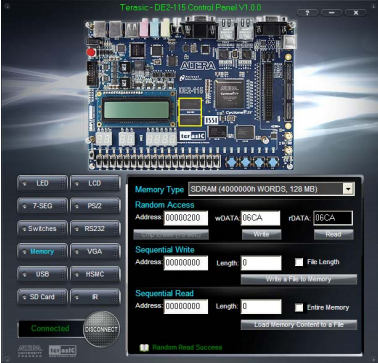
\includegraphics[width=100mm]{Lab5/figures/controlpanel.png}
	\caption{DE2-115 Control Panel - Accessing SDRAM/FLASH/EEPROM Menu}
	\label{fig:controlpanel}
\end{figure}

\subsubsection{FLASH Memory Controller}
The Altera DE2-115 FPGA Development Board contains an 8 MB FLASH memory chip. For this activity you will implement a FLASH memory controller that can read and write to the first 256 bits of the chip. A list of pins used for interacting with the chip can be found in Table \ref{tab:flash}. Notice that addresses are normally 23 bits long however for this exercise you should set FL\_ADDR[19] to FL\_ADDR[22] to the source address and set the remaining bits to zero. 

You should pay careful attention to how data is read and written to the chip. The signal FL\_CE\_N should be kept HIGH to keep the chip enabled. If you want to read data from the chip, you must first tell the chip the address of where the data is stored and then set the signal FL\_OE\_N to HIGH in order to send the data onto the data lines. Once the data is read, set the signal FL\_OE\_N back to LOW. If you want to write data to the chip, you must tell the chip the address location and set the data on the data lines then set FL\_WE\_N to HIGH. When the operation is completed, make sure to set the signal FL\_WE\_N to LOW. NOTE: you should never set both FL\_OE\_N and FL\_WE\_N to HIGH at the same time as you may damage the device. FL\_RY may be useful to determine if an operation has been completed. 

\begin {table}[H]
	\caption {Signal assignments for interfacing with the flash memory chip} 
	\label{tab:flash} 
	\begin{center}
    		\begin{tabular}{ | c | c |}
			\hline
 			{\bf Signal} & {\bf Description} \\ \hline
			FL\_ADDR[0] to FL\_ADDR[22] & FLASH Address[0] to FLASH Address[22] \\ \hline
			FL\_DQ[0] to FL\_DQ[7] & FLASH Data[0] to FLASH Data[7] \\ \hline
			FL\_CE\_N & FLASH Chip Enable (set HIGH)\\ \hline
			FL\_OE\_N & FLASH Output Enable \\ \hline
			FL\_RST\_N & FLASH Reset (set LOW)\\ \hline
			FL\_RY & FLASH Ready/Busy output \\ \hline
			FL\_WE\_N & FLASH Write Enable \\ \hline
			FL\_WP\_N & Flash Write Protect (set LOW)\\ 
			\hline
    		\end{tabular}
	\end{center}
\end{table}

\subsubsection{Results Display}
As has been done in previous labs, create a display driver for showing information relative the the current state.

\begin{itemize}
	\item HEX7 and HEX6 should display the value stored in Source Address 1. 
	\item HEX5 and HEX4 should display the value stored in Source Address 2.
	\item HEX3 and HEX2 should display the result of the operation.
	\item HEX0 should display the Program Counter
	\item LEDG3 through LEDG0 should display the current state; FETCH, DECODE, EXECUTE, and MEMORY\_WRITE respectively. 
	\item The display should reset to a dashes if the data is not available yet.
\end{itemize}


\subsection{Lab Report}
After completing the activities in this lab you should create a zip folder with the following and then submit it to Sakai:

\begin{itemize}
	\item Commented VHDL code.
	\item VHDL test bench with at least one instruction for all 8 operations.
	\item Photos of results from the test bench
	\item This processor is single-cycle which means it can only run one instruction at a time, how would you make the processor run in parallel? How many instructions can theoretically be worked on at the same time? Provide a diagram along with a written response.
	\item A discussion on the results of compilation including longest path delay, the total number of logic elements used, and issues you encountered while performing the lab.
\end{itemize}